\documentclass[addpoints]{exam}

\usepackage{amsmath}
\usepackage{hyperref}
\usepackage{tikz}
\usepackage{pseudocode}

% Header and footer.
\pagestyle{headandfoot}
\runningheadrule
\runningfootrule
\runningheader{CS 201 DS II}{Homework 5a}{Spring 2018}
\runningfooter{}{Page \thepage\ of \numpages}{}
\firstpageheader{}{}{}

\qformat{{\large\bf Exercise \thequestiontitle}\hfill[\totalpoints\ points]}
\boxedpoints
\printanswers

\title{\textbf{\tt Habib University}\\ \textbf{\tt CS 201 Data Structures II}\\ \textbf{\tt Spring 2018}}
\author{\textbf{\tt Emad Bin Abid - Saman Gaziani}\\ {\tt $Team: hw-5a-sg02494-ea02893-5$}}
\date{\textbf{\tt Homework 5a}\\ \textbf{\tt Submitted: March 23\textsuperscript{rd}, 2018}}

\begin{document}
\maketitle

\begin{questions}

  \titledquestion{6.4*}[10]
  Implement a non-recursive method, {\tt size2(u)}, that computes
  the size of the subtree rooted at node {\tt u}.
  \begin{solution}\\ \\
  	Assuming that the given tree is a binary tree. \\ \\
  	\begin{pseudocode}{size}{G, u}
  		\label{Size}
  		\COMMENT{Finds the size of a subtree $T$ rooted at $u$.}\\
  		
  		\PROCEDURE{size2}{$u$}
  		\IF u \neq NULL
		\THEN
		\BEGIN
		size \GETS 0 \\
		queue \GETS [$ $]\\
		queue.add(u)\\ \\
		
			\WHILE queue \neq [$ $] \DO 
  			\BEGIN
  				b \GETS queue.dequeue()\\
  				size \GETS size + 1\\ \\
  				
  				\IF b.left \neq NULL
  				\THEN 
  					queue.add(b.left)\\
  				
  				\IF b.right \neq NULL
  				\THEN 
  					queue.add(b.right)\\ 
	  		\END \\ \\
	  		\RETURN{size}
		\END \\
  		\ENDPROCEDURE
  	\end{pseudocode}
  \end{solution}
\pagebreak

  \titledquestion{6.9}
  The pre/in/post-order numbering of a tree labels the nodes of a tree with the integers $0,\ldots,n-1$ in the order that they are encountered by a pre/in/post-order traversal. See \href{http://opendatastructures.org/ods-python/6_3_Discussion_Exercises.html#fig:binarytree-numbering}{Figure 6.10} in the book for an example.

  Suppose we are given a binary tree with pre-, post-, and in-order numbers assigned to the nodes. Show how these numbers can be used to answer each of the following questions in constant time.
  \begin{parts}
    \part[10] Given a node $u$, determine the size of the subtree rooted at $u$.
  \begin{solution}\\ \\
  	//Error 404: Answer not found!
  \end{solution}
    \part[10] Given a node $u$, determine the depth of $u$.
  \begin{solution}\\ \\
  	//Error 404: Answer not found!
  \end{solution}
    \part[10] Given two nodes $u$ and $w$, determine if $u$ is an ancestor of $w$.
  \begin{solution}\\ \\
  	To find whether $w$ is in the subtree of $u$, we check pre-order number of $u$, the post-order number of $u$, the pre-order number of $w$ and the post-order number of $w$. If we come up with a result that pre-order number of $w$ is larger than pre-order number of $u$ and post-order number of $w$ is less than post-order number of $u$ then we get our required result and hence it can be said that $w$ is in the sub-tree of $u$.
  \end{solution}
  \end{parts}
\pagebreak

  \titledquestion{6.15}[10]
  Describe how to add the elements $\{1,\ldots,n\}$ to an initially empty BST in such a way that the resulting tree has height $n-1$. How many ways are there to do this?
  \begin{solution}\\ \\
  	Let there be an initially empty binary search tree, $T$. Moreover, let there be a pool $P$ of $n$ values namely; $1, 2, 3, \ldots, n$ which need to be added as node values in $T$. In order to maintain the height $n-1$ for $T$, at every stage we either add the least value or the highest value from the remaining pool of values. Assuming that our pool of values is sorted in an ascending order, we either add the first value from the pool or the last value from the pool. We recursively follow the process until we remain with just one value in the pool. \\ \\
  	Following the process above, each possibility to generate a tree of height $n-1$ further has two possibilities (least or highest) for a particular node position. For a particular tree, at each stage there are two possibilities and since there will be $n-1$ such stages, therefore, the total number of ways to add the elements in an initially empty $BST$ turn out to be $2^{n-1}$.
  \end{solution}
\pagebreak

  \titledquestion{7.3}[10]
  Prove the assertion that there are 21,964,800 sequences that generate the tree on the right hand side of \href{http://opendatastructures.org/ods-python/7_1_Random_Binary_Search_Tr.html#fig:rbs-lvc}{Figure 7.1} in the book. (Hint: Give a recursive formula for the number of sequences that generate a complete binary tree of height $h$ and evaluate this formula for $h = 3$.)
  \begin{solution}\\ \\
  	Since, the tree given in figure 7.1 is a tree in which all leaf nodes have the same height $h$, we recursively find the number of ways in which the sequence will generate the same Binary Search Tree as given in the figure. We recursively traverse through the left and right subtrees starting at the root node. The recursive relation is given as, \\ 
  	\begin{center}
  		$num\_ways(T, h) = num\_ways(T_L, h-1) \times num\_ways(T_R, h-1) \times IW$
  	\end{center}
  	where, $IW = $ interleaved ways.\\ \\
  	The question here arises, how do we compute the factor $IW$? We do this by the following formula,\\
  	\begin{center}
  		$\dfrac{(a+b)!}{a! \times b!}$
  	\end{center}
  	where, $a$ and $b$ are the nodes in left and right subtrees. \\ \\
  	Base case for recursive steps -- $num\_ways(T, 1)=2$\\ 
  	Testing it for $h=3$ we get, \\
  	\begin{center}
  		$num\_ways(T, 3) = num\_ways(T_L, 2) \times num\_ways(T_R, 2) \times \dfrac{(a+b)!}{a! \times b!}$\\
  		$num\_ways(T, 2) = num\_ways(T_L, 1) \times num\_ways(T_R, 1) \times \dfrac{(a+b)!}{a! \times b!}$\\
  	\end{center}
  	Now,\\
  	\begin{center}
  		$num\_ways(T, 2) = 2 \times 2 \times \dfrac{(3+3)!}{3! \times 3!}$\\
  		$num\_ways(T, 2) = 80$\\
  	\end{center}
  	Since the tree is symmetric, $num\_ways(T_L, 2) = num\_ways(T_R, 2) = 80$\\ \\
  	Therefore, 
  	\begin{center}
  		$num\_ways(T, 3) = 80 \times 80 \times \dfrac{(7+7)!}{7! \times 7!}$\\
  		$num\_ways(T, 3) = 21964800$
	\end{center}  	  
  	Hence, proved.
  	\\ \\
  	\textbf{\underline{Note:}} The idea of this question is taken from \href{https://stackoverflow.com/questions/17119116/how-many-ways-can-you-insert-a-series-of-values-into-a-bst-to-form-a-specific-tr}{stackoverflow}
  \end{solution}
\pagebreak

  \titledquestion{7.7}
  Suppose that a binary search tree stores, at each node, {\tt u}, the height, {\tt u.height}, of the subtree rooted at {\tt u}, and the size, {\tt u.size} of the subtree rooted at {\tt u}.
  \begin{parts}
  \part[10] Show how, if we perform a left or right rotation at {\tt u}, then these two quantities can be updated, in constant time, for all nodes affected by the rotation.
  \begin{solution}\\ \\
  	The \textbf{\textit{height}} of a node is the number of edges on the longest path from the node to a leaf. For instance, a leaf node will have a height of 0.\\ \\
	Since the height of any node in a tree is measured w.r.t. the leaf node of that particular branch, the heights of all the nodes remain un-affected apart from two nodes; the node $n$ on which rotation is performed, and the k-node where $k$ is the immediate child of $n$ and lies on the opposite of rotated side (left or right) of $n$. The reason these two nodes are affected is because the new height of original node $n$ will be one plus the height of that $n$'s child which is on the side of rotation. Plus, the new height of k-node will be the maximum between $k$'s previous height and $n$'s new height + 1. Since the height of only these two nodes will be altered, we can change them in constant time. Hence, the purpose of changing the height is achieved in constant time. \\ \\
	For updating the size, it is clear that size of $k$ will become the size of $n$. Therefore,
	\begin{center}
		$k.size = n.size$
	\end{center}
	Moreover, the size of $n$ will alter in such a fashion that its new size becomes the size of its immediate child on the side of rotation plus the size of immediate child of $k$ which changes its parent after rotation. Plus one is also done to accommodate the node $n$ itself. 
	\begin{center}
		$n.size = n\_ichild.size + 1 + k\_ichild.size$
	\end{center}
	where, $n\_ichild.size$ = size of immediate child of $n$ on the side of rotation\\
	and,  $k\_ichild.size$ = size of immediate child of $k$ which changes its parent after rotation\\ \\
	Both updates can be shown via an example given below:\\ \\
	\textbf{Before Rotation:}\\
	\begin{center}
		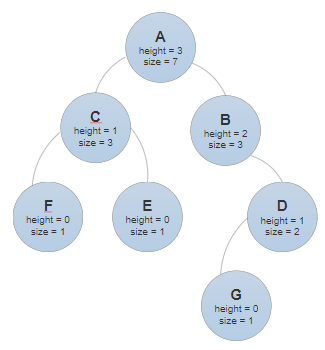
\includegraphics[scale=0.7]{question_7point7a_1.png}\\
	\end{center}
\pagebreak
	\textbf{After Rotation:}\\
	\begin{center}
		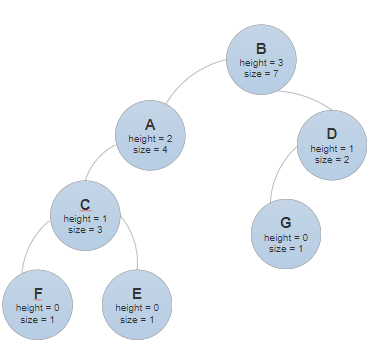
\includegraphics[scale=0.7]{question_7point7a_2.png}\\
	\end{center}
	\textbf{\underline{Note}:} The definition of height of a tree is taken from \href{https://www.quora.com/What-is-the-difference-between-height-and-depth-of-a-tree}{Quora}.
  \end{solution}
\pagebreak  
  
  \part[10] Explain why the same result is not possible if we try to also store the depth, {\tt u.depth}, of each node {\tt u}.
  \begin{solution}
    The \textbf{\textit{depth}} of a node is the number of edges from the node to the tree's root node. For instance, a root node will have a depth of 0.
	\\ \\
	The same result is indeed not possible if we try to store the depth of each node. The reason lies in the definition of depth itself. Unlike height, where the leaf node had the same value 0, in case of storing depth each node can have a different depth. Having said this, there is not a common value of reference to gauge other nodes w.r.t. the leaf. And hence during the process of rotation the nodes change positions, there is no common leaf reference. This results in the change of depth values at many nodes. Hence, the update needs to be done in $O(n)$ because in the worst case, the depth of all $n$ nodes need to be updated. \\ \\
	The size may however be computed in constant time using the logic which was stated for height. 
	Both updates can be shown via an example given below:\\ \\
	\textbf{Before Rotation:}\\
	\begin{center}
		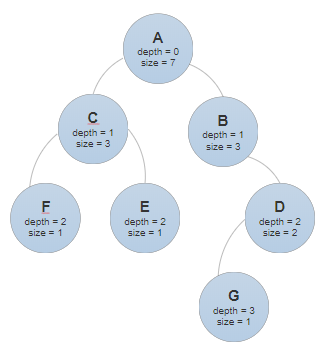
\includegraphics[scale=0.6]{question_7point7b_1.png}\\
	\end{center}
	
	\textbf{After Rotation:}\\
	\begin{center}
		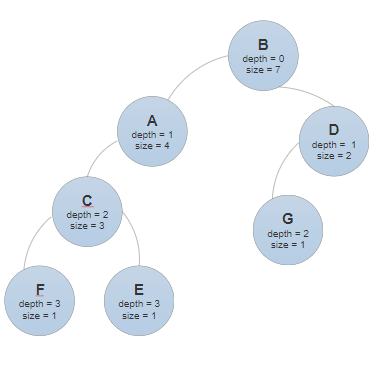
\includegraphics[scale=0.6]{question_7point7b_2.png}\\
	\end{center}
	\textbf{\underline{Note}:} The definition of depth of a tree is taken from \href{https://www.quora.com/What-is-the-difference-between-height-and-depth-of-a-tree}{Quora}.
  \end{solution}
\end{parts}
\pagebreak

\end{questions}

* - The question has been modified from the one in the book.

\end{document}